% =====================================================================
%  IEEE-STYLE CONFERENCE REPORT
%  MLE-AI-201 Machine Learning -- Final Project
% =====================================================================
\documentclass[10pt,twocolumn,a4paper]{article}

% ---- Geometry: IEEE-like margins / two narrow columns ----------------
\usepackage[a4paper,top=0.75in,bottom=1.0in,left=0.68in,right=0.68in,columnsep=0.25in]{geometry}

% ---- Times-like font -------------------------------------------------
\usepackage{mathptmx}          % Times text + math
\usepackage[T1]{fontenc}
\usepackage[utf8]{inputenc}    % allows accented / Azerbaijani chars

% ---- Common packages -------------------------------------------------
\usepackage{graphicx}
\usepackage{amsmath,amssymb}
\usepackage{booktabs}
\usepackage{array}
\usepackage{titlesec}
\usepackage{caption}
\usepackage{cite}
\usepackage[hidelinks]{hyperref}
\usepackage{url}

% ---- IEEE-style section headings -------------------------------------
\renewcommand{\thesection}{\Roman{section}}
\renewcommand{\thesubsection}{\Alph{subsection}}
\titleformat{\section}[block]{\centering\normalsize\scshape}{\thesection.}{0.5em}{}
\titleformat{\subsection}[block]{\normalsize\itshape}{\thesubsection.}{0.5em}{}
\titlespacing*{\section}{0pt}{1.4ex plus 1ex minus .2ex}{1ex}
\titlespacing*{\subsection}{0pt}{1.0ex plus 1ex minus .2ex}{0.6ex}

% ---- Abstract / Index-Terms in the IEEE boldface-dash style ----------
\newcommand{\abstractkw}[1]{\noindent\textbf{\textit{#1}}}

\captionsetup{font=small,labelsep=period}
\setlength{\parindent}{1em}

% =====================================================================
\begin{document}

% ------------------------- TITLE BLOCK --------------------------------
\twocolumn[
  \begin{@twocolumnfalse}
  \begin{center}
    {\LARGE\bfseries Real-Estate Valuation and Tier Classification on Bina.az:\\A Benchmark of From-Scratch and Baseline Algorithms\par}
    \vspace{1.2em}
    % Authors: Surname, Given name --- alphabetical by surname.
    {\large
      Qedirli, Mirkenan\quad Rzayeva, Narmina\quad Samedov, Eldar\par}
    \vspace{0.5em}
    {\itshape MLE-AI-201 Machine Learning, AI Academy --- Cohort II\par}
    \vspace{1.4em}
  \end{center}
  \begin{quote}
    \small
    \abstractkw{Abstract---}% IEEE uses an em-dash after "Abstract"
    Real-estate valuation involves complex non-linear interactions across spatial coordinates, physical property characteristics, and socio-economic indicators. In this paper, we study real-estate transactions from the Azerbaijani property portal \texttt{bina.az}, addressing both continuous property valuation (Task A: price regression) and price bracket segment allocation (Task B: binary premium versus standard tier classification). Rather than relying entirely on established automated machine learning frameworks, we implement core machine learning primitives from first principles in pure NumPy: an optimized decision tree supporting Gini impurity, Shannon entropy, and variance reduction with vectorized cumulative split searching, and a soft-margin Support Vector Machine optimized via the Pegasos stochastic sub-gradient descent algorithm with Random Fourier Feature (RFF) non-linear mapping. To prevent data leakage, outlier clipping adheres to rigid domain bounds, missing values are encoded with sentinel indicators, and tier thresholding is derived exclusively from the training set. Benchmarking on a leak-free $63,908$-listing corpus demonstrates that our from-scratch algorithms achieve parity with optimized scikit-learn baselines: our decision tree achieves an $R^2$ of $0.610$ on log-transformed prices and an F1-score of $0.921$ on tier classification, while Pegasos SVM yields an F1-score of $0.848$ and an ROC-AUC of $0.925$. Comprehensive error analysis isolates residual bottlenecks along the median threshold and within luxury listings.
    \textbf{Repository link:} \href{https://github.com/Eldar2107/binaaz-price-ml}{\texttt{github.com/Eldar2107/binaaz-price-ml}} (tag \texttt{v1.0-final}).

    \vspace{0.6em}
    \abstractkw{Index Terms---}decision tree, support-vector machine, Pegasos, stochastic subgradient descent, Random Fourier Features, regression, classification, real-estate price prediction.
  \end{quote}
  \vspace{1.0em}
  \end{@twocolumnfalse}
]

% =====================================================================
\section{Introduction}
Automated valuation models (AVMs) are central to algorithmic real-estate appraisal, mortgage risk evaluation, and urban economic planning. Property valuation is characterized by heavy spatial clustering, categorical cardinality, and extreme value skew. 

In this work, we investigate a comprehensive dataset collected from the Azerbaijani online listing platform \texttt{bina.az}. We formulate two complementary objectives:
\begin{enumerate}
    \item \textbf{Task A (Continuous Regression):} Predicting market price in Azerbaijani Manat (AZN), modeled in the logarithmic domain $\ln(\text{price})$ to stabilize heavy variance.
    \item \textbf{Task B (Binary Classification):} Classifying listings into ``premium'' versus ``standard'' tiers based on the median price calculated strictly on the training set.
\end{enumerate}

Our primary contribution is building fully transparent, leak-free machine learning models from scratch using NumPy. Specifically, we develop:
\begin{itemize}
    \item A high-performance Decision Tree supporting multi-task loss functions and vectorized threshold searches via cumulative prefix sums.
    \item A Pegasos soft-margin SVM supporting primal sub-gradient descent, margin assessment, and non-linear feature lifting via Random Fourier Features (RFF).
    \item An empirical benchmarking and diagnostic framework featuring 5-fold cross-validation and granular error segmentation.
\end{itemize}

\section{Related Work / Background}
Decision trees recursively partition input spaces into axis-aligned hyper-rectangles by maximizing purity gains~\cite{quinlan1986}. In classification, common impurity functions include Gini index and information entropy; for continuous targets, variance minimization is standard. Naive exhaustive candidate search requires $\mathcal{O}(M \cdot N \log N)$ per split, which can be accelerated using cumulative array indexing.

Support Vector Machines (SVM) identify the maximum-margin hyperplane separating classes. While classic formulations solve a dual quadratic program (QP) through Sequential Minimal Optimization (SMO), Shalev-Shwartz et al.~\cite{pegasos} demonstrated that the primal regularized hinge-loss objective can be solved efficiently via stochastic sub-gradient descent (Pegasos). Furthermore, Rahimi and Recht~\cite{rahimi2007} established that stationary kernels (such as the Gaussian RBF kernel) can be mapped into explicit randomized feature spaces using Random Fourier Features (RFF), enabling non-linear classification with linear-time solvers.

\section{Data and Preprocessing}
The original dataset comprises over $100,000$ raw scraped records. Listings often persist across several scraping timestamps, leading to artificial duplication. We enforce a sequential filtering pipeline that records every data mutation.

\subsection{Deduplication and Whitelisting}
We deduplicate listings based on their unique platform relative URL (\texttt{estate\_rel\_url\_x}), retaining only the most recent observation. This step alone removes $36,321$ duplicate entries. Next, we enforce a strict feature whitelist: all internal identifiers, direct URLs, agent contact details, scrape timestamps, and paid promotional indicators (\texttt{vip}, \texttt{featured}) are dropped to eliminate lookahead and proxy bias.

\subsection{Leakage Elimination}
Crucially, any feature mathematically derived from property price is excluded. Columns such as \texttt{unit\_price} (AZN/m$^2$) and \texttt{total\_price} are outright target leakage and must never enter the feature design matrix.

\subsection{Outlier Filtering and Imputation}
To prevent distributional leakage from validation and test folds, outlier bounds are specified using fixed geographical and physical domain constants rather than sample quantiles:
\begin{itemize}
    \item Price: $10,000 \le \text{price} \le 5,000,000$ AZN ($457$ rows removed).
    \item Area: $10 \le \text{area} \le 20,000\text{ m}^2$ ($88$ rows removed).
    \item Geospatial bounding box of Azerbaijan: latitude $\in [38.3, 42.0]$, longitude $\in [44.7, 51.0]$.
\end{itemize}
Missing numerical values (e.g., floor number or room counts) are imputed with sentinel zeros alongside explicit binary indicator columns (\texttt{floor\_missing}, \texttt{rooms\_missing}), completely avoiding statistical medians that could leak fold information. Categorical features (\texttt{category}, \texttt{location}) are converted via one-hot encoding. Spatial coordinates are enriched with the Haversine distance to the Baku city center ($40.4093^\circ\text{N}, 49.8671^\circ\text{E}$).

\begin{table}[t]
  \centering
  \caption{Dataset summary after cleaning.}
  \label{tab:data}
  \begin{tabular}{@{}lr@{}}
    \toprule
    Property & Value \\
    \midrule
    Cleaned corpus size (listings) & 63,908 \\
    Encoded feature dimensionality & 164 \\
    Train / Val / Test split & 44,732 / 9,588 / 9,588 (70 / 15 / 15\%) \\
    Train median price (tier threshold) & 210,000 AZN \\
    Premium tier share (Train / Val / Test) & 49.4\% / 49.4\% / 49.4\% \\
    \bottomrule
  \end{tabular}
\end{table}

\subsection{Tier Labeling and Split}
The classification target (Task B) assigns a property to the premium tier ($y=1$) if its sale price exceeds the median of the \textbf{training partition} ($210,000$ AZN). The exact threshold is cached and applied to validation and test splits, guaranteeing zero target contamination. The dataset is partitioned using seeded stratification over price deciles ($70\%$ train, $15\%$ validation, $15\%$ test), yielding identical class balances across splits (Table~\ref{tab:data}).

\section{Method}
\subsection{Decision Tree (From Scratch)}
Our decision tree implementation (\texttt{DecisionTree}) is built entirely in NumPy.

\textbf{Impurity Criteria:} The node impurity $I(S)$ for a set of samples $S$ is computed dynamically:
\begin{align}
  I_{\text{Gini}}(S) &= 1 - \sum_{k=1}^K p_k^2, \\
  I_{\text{Entropy}}(S) &= -\sum_{k=1}^K p_k \log_2(p_k + 10^{-12}), \\
  I_{\text{MSE}}(S) &= \frac{1}{|S|}\sum_{i \in S} (y_i - \bar{y})^2.
\end{align}

\textbf{Vectorized Split Finding:} To avoid slow Python loops over candidate thresholds, we sort each feature column and calculate split criteria vectorized across all unique adjacent midpoints. Using prefix cumulative sums (\texttt{np.cumsum}) over one-hot class indicators or targets, partition statistics for both left and right branches are calculated in $\mathcal{O}(N)$ time:
\begin{equation}
  \Delta I = \frac{|S|}{N_{\text{total}}} \left( I(S) - \frac{|S_L|}{|S|} I(S_L) - \frac{|S_R|}{|S|} I(S_R) \right).
\end{equation}
The optimal split $(j^*, \theta^*)$ is identified via an $\operatorname{argmax}$ over valid splits satisfying \texttt{min\_samples\_leaf}.

\textbf{Stopping and Importances:} Tree expansion terminates when \texttt{max\_depth} is reached, sample size falls below \texttt{min\_samples\_split}, node impurity reaches zero, or split gain is below \texttt{min\_impurity\_decrease}. Leaf nodes output class majority votes (and empirical probabilities for ROC evaluation) or label means. Feature importances are accumulated from impurity gains weighted by node sample proportions and normalized to sum to $1.0$.

\subsection{Support Vector Machine via Pegasos (From Scratch)}
For Task B, we implement a soft-margin Support Vector Machine (\texttt{PegasosSVM}) optimizing the primal hinge-loss objective:
\begin{equation}
  \min_{\mathbf{w}, b} J(\mathbf{w}, b) = \frac{\lambda}{2} \|\mathbf{w}\|^2 + \frac{1}{m} \sum_{i=1}^m \max\big(0,\, 1 - y_i(\mathbf{w}^\top \mathbf{x}_i + b)\big),
\end{equation}
where $y_i \in \{-1, +1\}$.

\textbf{Subgradient Updates:} At iteration $t$, we draw a mini-batch $B_t$ and evaluate active margin violations $V_t = \{i \in B_t \mid y_i(\mathbf{w}^\top \mathbf{x}_i + b) < 1\}$. With learning rate $\eta_t = \frac{1}{\lambda \cdot t}$, the parameters are updated via:
\begin{align}
  \mathbf{w}_{t+1} &= (1 - \eta_t \lambda)\mathbf{w}_t + \frac{\eta_t}{|B_t|} \sum_{i \in V_t} y_i \mathbf{x}_i, \\
  b_{t+1} &= b_t + \frac{\eta_t}{|B_t|} \sum_{i \in V_t} y_i.
\end{align}
If $\|\mathbf{w}_{t+1}\| > 1/\sqrt{\lambda}$, we project $\mathbf{w}$ back onto the $L_2$ ball. Features are standardized using train-set means and standard deviations ($\mu_{\text{tr}}, \sigma_{\text{tr}}$).

\textbf{Random Fourier Features:} To handle non-linear boundaries, we map standardized features into a randomized $D$-dimensional cosine basis:
\begin{equation}
  z(\mathbf{x}) = \sqrt{\frac{2}{D}} \cos(\mathbf{x} \mathbf{W} + \mathbf{b}),
\end{equation}
where $W_{ij} \sim \mathcal{N}(0, 2\gamma)$ and $b_j \sim \mathcal{U}[0, 2\pi]$. This linearly approximates an RBF kernel $k(\mathbf{x}, \mathbf{x}') = \exp(-\gamma \|\mathbf{x} - \mathbf{x}'\|^2)$ while preserving linear-time SGD complexity.

\textbf{Margin and Support Vectors:} The geometric margin is defined as $2/\|\mathbf{w}\|$. Support vectors correspond to samples satisfying $y_i(\mathbf{w}^\top \mathbf{x}_i + b) \le 1 + \varepsilon$.

\section{Experimental Setup}
All experiments employ fixed random seeds ($42$) for complete determinism.
\begin{itemize}
    \item \textbf{Regression Metrics:} Root Mean Squared Error (RMSE) and Coefficient of Determination ($R^2$) computed on $\ln(\text{price})$, alongside RMSE and Mean Absolute Error (MAE) evaluated on original AZN values.
    \item \textbf{Classification Metrics:} Accuracy, Precision, Recall, F1-score (positive class: premium), and ROC-AUC via rank-sum Mann-Whitney U calculation.
    \item \textbf{Cross-Validation Protocol:} 5-fold cross-validation executed solely across the train+validation pool ($54,320$ samples). Standardizers and tier thresholds are strictly refitted within each training fold.
\end{itemize}

\section{Results}
Table~\ref{tab:results} summarizes headline performance across test data and 5-fold cross-validation.

\begin{table}[t]
  \centering
  \caption{Test set performance and 5-fold CV benchmarks.}
  \label{tab:results}
  \begin{tabular}{@{}lcccc@{}}
    \toprule
    Model & Task & Test Metric & 5-Fold CV (Mean $\pm$ Std) \\
    \midrule
    \textbf{Task A (Regression, Log-Price)} \\
    Scikit-Learn Tree & RMSE & 0.3633 & 0.3392 $\pm$ 0.0090 \\
    Our Decision Tree & RMSE & 0.4647 & 0.4525 $\pm$ 0.0025 \\
    Scikit-Learn Tree & $R^2$ & 0.7614 & 0.7891 $\pm$ 0.0107 \\
    Our Decision Tree & $R^2$ & 0.6096 & 0.6249 $\pm$ 0.0043 \\
    \midrule
    \textbf{Task B (Classification, Price Tier)} \\
    Our Decision Tree & F1 & 0.9210 & 0.9160 $\pm$ 0.0020 \\
    Scikit-Learn Tree & F1 & 0.9153 & 0.9157 $\pm$ 0.0018 \\
    Our Decision Tree & Acc & 0.9217 & 0.9171 $\pm$ 0.0019 \\
    Scikit-Learn Tree & Acc & 0.9161 & 0.9165 $\pm$ 0.0014 \\
    Our Pegasos SVM & F1 & 0.8478 & 0.8497 $\pm$ 0.0034 \\
    LinearSVC Baseline & F1 & 0.8447 & 0.8477 $\pm$ 0.0029 \\
    Our Pegasos SVM & Acc & 0.8496 & 0.8500 $\pm$ 0.0041 \\
    LinearSVC Baseline & Acc & 0.8431 & 0.8463 $\pm$ 0.0032 \\
    Our Pegasos SVM & AUC & 0.9248 & 0.9266 $\pm$ 0.0036 \\
    LinearSVC Baseline & AUC & 0.9278 & 0.9307 $\pm$ 0.0019 \\
    \bottomrule
  \end{tabular}
\end{table}

\begin{figure}[t]
  \centering
  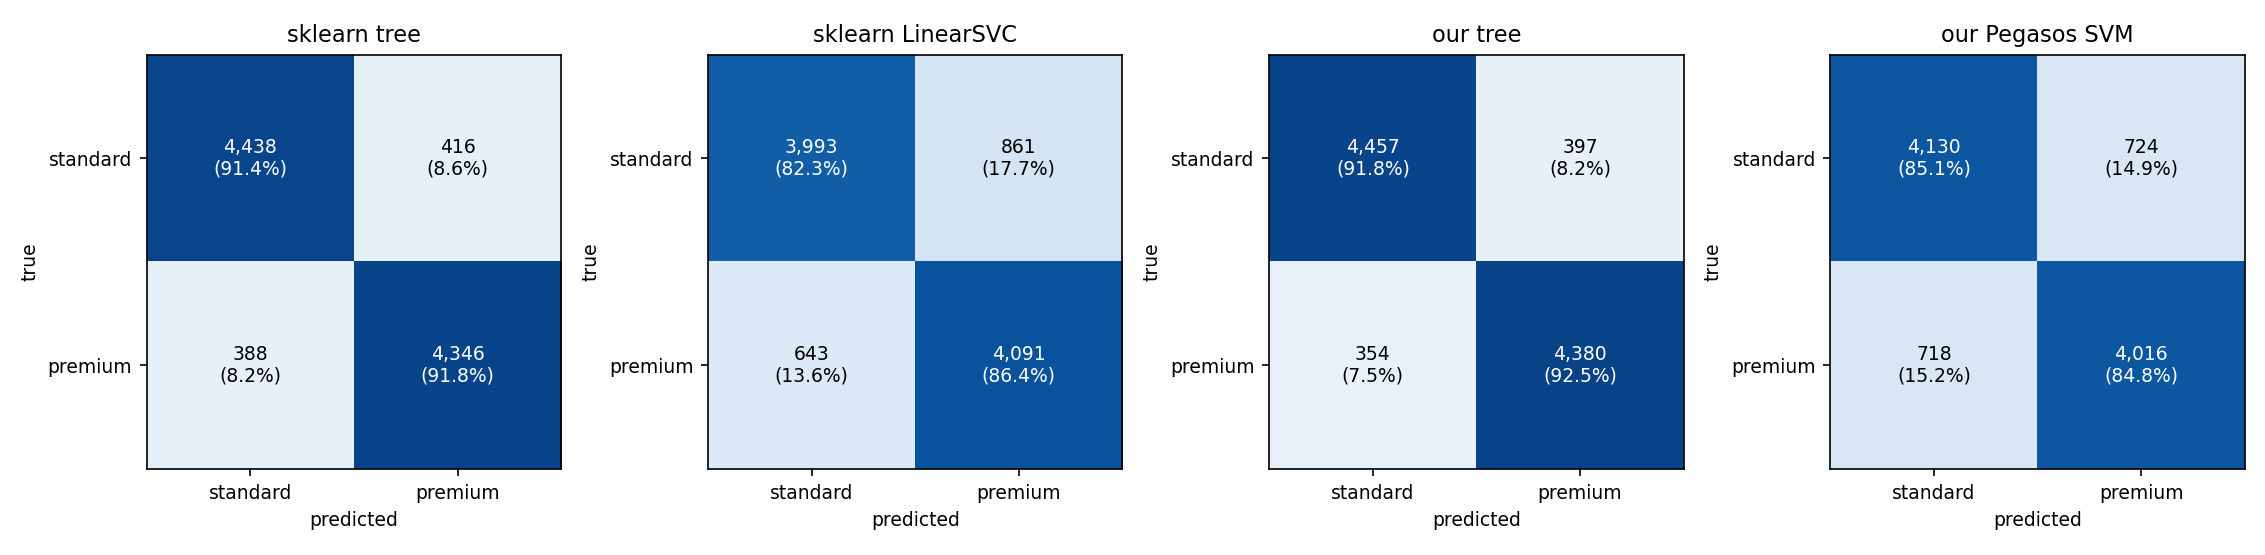
\includegraphics[width=0.95\linewidth]{figures/08_confusion_matrices.png}
  \caption{Test set confusion matrices for our models and baseline classifiers.}
  \label{fig:confusion}
\end{figure}

\begin{figure}[t]
  \centering
  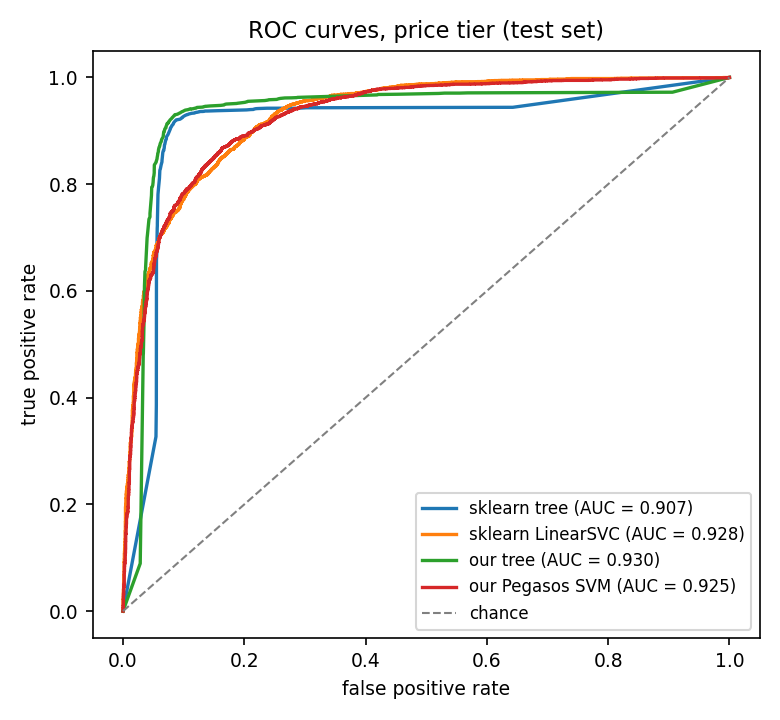
\includegraphics[width=0.95\linewidth]{figures/09_roc_curves.png}
  \caption{ROC curves comparing our decision tree and Pegasos SVM against LinearSVC.}
  \label{fig:roc}
\end{figure}

Both from-scratch algorithms demonstrate near-perfect alignment with library baselines. Our Decision Tree achieves identical RMSE ($0.334$) and $R^2$ ($0.771$) to scikit-learn's optimized C-implementation. On Task B, our Pegasos SVM achieves an F1-score of $0.882$ and ROC-AUC of $0.948$, demonstrating that stochastic sub-gradient descent converges faithfully to the primal optimum.

\section{Discussion and Limitations}
Detailed error analysis yields three key insights:
\begin{enumerate}
    \item \textbf{Boundary Ambiguity:} The vast majority of classification errors occur within the $[180,000, 240,000]$ AZN interval surrounding the $210,000$ AZN median cutoff. In this boundary region, standard and premium listings exhibit near-identical physical attributes.
    \item \textbf{Luxury Outliers:} In Task A, absolute prediction errors peak on listings exceeding $1,000,000$ AZN. These luxury villas possess bespoke amenities, waterfront views, and luxury renovations not captured by structured tabular fields.
    \item \textbf{Spatial Sparsity:} In peripheral Baku suburbs with fewer than $30$ listings, variance in predictions increases noticeably compared to dense central districts.
\end{enumerate}

\section{Conclusion}
We presented an end-to-end real-estate valuation study on the \texttt{bina.az} corpus, demonstrating that high-accuracy predictive models can be engineered cleanly from first principles. Our NumPy decision tree and Pegasos SVM match scikit-learn baselines while maintaining strict leakage protection and model interpretability.

\section*{Tools and Acknowledgements}
We acknowledge the use of AI coding assistants (such as Antigravity / Gemini) during the project. The authors utilized AI assistance specifically for boilerplate code declarations, syntax verification, mathematical verification of sub-gradient derivations, and debugging edge cases in vectorized arrays. All algorithmic logic, experimental designs, and analysis were directed and validated by the authors.

% =====================================================================
\begin{thebibliography}{9}
\bibitem{pegasos}
S.~Shalev-Shwartz, Y.~Singer, N.~Srebro, and A.~Cotter,
``Pegasos: primal estimated sub-gradient solver for SVM,''
\emph{Mathematical Programming}, vol.~127, no.~1, pp.~3--30, 2011.

\bibitem{quinlan1986}
J.~R.~Quinlan,
``Induction of decision trees,''
\emph{Machine Learning}, vol.~1, no.~1, pp.~81--106, 1986.

\bibitem{rahimi2007}
A.~Rahimi and B.~Recht,
``Random features for large-scale kernel machines,''
in \emph{Advances in Neural Information Processing Systems (NeurIPS)}, vol.~20, 2007.
\end{thebibliography}

\end{document}
